    \documentclass[12pt]{report}
\usepackage{amsmath}
\usepackage{lscape}
\usepackage{graphicx}

\setlength {\marginparwidth }{2cm}
\usepackage[colorinlistoftodos]{todonotes}

\usepackage{graphicx}
\usepackage{multirow}
\usepackage{multicol}
\usepackage{caption}
\usepackage{subcaption}

\usepackage[english]{babel}
\usepackage{wrapfig}
\usepackage{lscape}
\usepackage{rotating}
\usepackage{epstopdf}
\bibliographystyle{IEEEtran}
\nocite{*}

% Fancy heading on all pages
\usepackage{fancyhdr}
\usepackage[fit]{truncate}
\pagestyle{fancy}
\fancyhead[OR]{\nouppercase{\truncate{0.7\headwidth}{\rightmark}}}
\fancyhead[OC, OL]{}


\usepackage{hyperref} 
\usepackage{ragged2e}


\def\skipspace{\vskip1em}

\newcommand{\say}[1]{``#1''}

\begin{document}

% \setcounter{chapter}{4}

\newcommand{\university}{Netaji Subhas University of Technology}
\newcommand{\department}{Computer Science and Engineering}

\begin{titlepage}
 \begin{center}
		
\includegraphics[width=0.30\textwidth]{images/logo.png}\\
		\normalsize
		% \sffamily

		\vspace{0.5cm}

		\Huge
		\textbf{Knowledge Representation in Cognitive Systems}
		\normalsize

		\vfill
		\textbf{\large Thesis } \\
		\vspace{0.6cm}

		Course: \\ \textbf{Cognitive Systems}\\
		% \vfill
		\vspace{0.8cm}


		Course Code: \\ \textbf{CICPE08}\\
		\vspace{0.8cm}
		Prepared by: \\
		\large
		\textbf{Shubhveer Singh Chaudhary (2021UCI8034)\\
  Kushagra Lakhwani (2021UCI8036)\\
  Vansh Kandwal (2021UCI8041)\\
  Sushant Lavania (2021UCI8061)}\\

		\normalsize
		\vspace{0.8cm}
		Supervised by:\\
		\large
		\textbf{Dr.Shobha Bhatt}\\
		\vspace{0.3cm}
		\normalsize

		\vfill
		% Department: \\
		\large
		\textbf{\department} \\

		\normalsize
		\vfill
		\textsc{\large \university}\\[1ex]
		{\large \today}
	\end{center}
\end{titlepage}



\tableofcontents

\addcontentsline{toc}{chapter}{Abstract}
\center\textbf{\large Abstract}

\begin{justify}
	The practical lab report \textit{``Operating Systems''} is the original and unmodified content submitted by \textit{Kushagra Lakhwani} (Roll No. 2021UCI8036).

	The report is submitted to \textit{Dr. Manoj Kumar} Department of Computer Science and Engineering, NSUT, Delhi, for the partial fulfillment of the requirements of the course \textit{``Operating Systems''} (CICPC09).
\end{justify}

\pagebreak

%\addcontentsline{toc}{chapter}{Certificate}
%%\thispagestyle{empty}
\chapter*{Certificate}

\begin{justify}
	This is to certify that the project progress report entitled \textbf{``\@title"} which is being submitted by \textbf{<TODO>}
	Dept. of Computer Science and Engineering \textbf{<TODO>} and (\textbf{<ROLL. NO>}) in partial fulfillment of the requirement for the degree
	of Master of Engineering in Electronics and Telecommunication Engineering with
	specialization <TODO>, has been prepared by him, under my
	supervision and guidance.\\[2cm]
\end{justify}

\begin{flushleft}
	Countersigned by:\\[4cm]
\end{flushleft}

\begin{minipage}{0.45\textwidth}
	\begin{flushleft} \large
		\emph{………………}\\
		HOD NAME \\
		Head of Dept.\\
		Dept. of E.T.C.,\\
		IIEST, Shibpur.\\
	\end{flushleft}
\end{minipage}
~
\begin{minipage}{0.45\textwidth}
	\begin{flushright} \large
		\emph{………………}\\

		Dean of Academic Affairs\\
		Dept. of Computer Science and Engineering\\

	\end{flushright}
\end{minipage}



\newpage
\listoffigures
\newpage
% \listoftables
% \newpage

\chapter{What is Knowledge}
\section{Introduction}
This is an example of the \texttt{pracjourn} document class.
Articles should always start with a section title, which will usually be `Introduction' or somesuch.

This document demonstrates the features of the document class.
Here are some logos and abbreviations:
\note{Tuned for Palatino, but refinements welcomed.}
\TeX, \pdfTeX, \BibTeX,\\ \MF, \MP, \LaTeX, \LaTeXe,
\mbox{\ConTeXt}, \pdfLaTeX, \XeTeX, \PracTeX, \TPJ, \PS.

On the following pages are shown the document divisions and list environments.

\section{Section headings}
\itshape The fact is that his precocity in vice was awful. At five months of age he
used to get into such passions that he was unable to articulate. At six
months, I caught him gnawing a pack of cards. At seven months he was in
the constant habit of catching and kissing the female babies. At eight
months he peremptorily refused to put his signature to the Temperance
pledge.
\note{Text from Edgar Allen Poe's `Never bet the Devil your head'.}

\subsection{Subsection}

Poverty was another vice which the peculiar physical deficiency of
Dammit's mother had entailed upon her son. He was detestably poor, and
this was the reason, no doubt, that his expletive expressions about
betting, seldom took a pecuniary turn. I will not be bound to say that I
ever heard him make use of such a figure of speech as ``I'll bet you a
dollar.'' It was usually ``I'll bet you what you please,'' or ``I'll bet you
what you dare,'' or ``I'll bet you a trifle,'' or else, more significantly
still, \emph{``I'll bet the Devil my head.''}

\subsubsection{Subsubsection}


\upshape Subsubsections are in the same font size as the body text, so I guess
it's possibly a little small. I doubt many people really will wish to
use a subsubsection in a journal article. But if they wish, there's
nothing stopping 'em.

\note{Another footnote test.
	This one has to be really long to see what happens
	when a footnote extends over more than one line.
	I.e., two or more.}

\begin{figure}[!ht]
	\centering test
	\caption{test}
\end{figure}

\paragraph{Paragraphs} Named paragraphs are very similar to description lists; however, these may be useful more \emph{multiple} paragraphs, whereas description lists work better with only a single paragraph per item.

\subparagraph{Subparagraphs} For those who want them\dots.

\section{Lists}
An itemized list:
\begin{itemize}
	\item one,
	\item two, and
	\item three.
	      A nested itemised list:
	      \begin{itemise}
		      \item one,
		      \item two, and
		      \item three.
	      \end{itemise}
\end{itemize}
An enumerated list:
\begin{enumerate}
	\item one,
	\item two, and
	\item three.
\end{enumerate}
A description list:
\begin{description}
	\item [one] the first,
	\item [two] the second, and
	\item [three] the third. A nested description list:
	      \begin{description}
		      \item [one] the first,
		      \item [two] the second, and
		      \item [three] the third.
	      \end{description}
\end{description}


\chapter{Knowledge Representation}

Data is like Lego blocks for the cognitive system, if our cognitive system can
learn to organize or put these blocks together into correct places then it is
termed as information, if this structure of data (blocks) can be used for
future use it is termed as knowledge.

\begin{enumerate}
  \item \textbf{Data}: Raw facts, figures, data that does not mean anything
    independently, much like individual LEGO blocks.

  \item \textbf{Information}: When data is organized, structured, or given
    context, it becomes information. Much like fitting LEGO blocks into a
    structure. Information gives logic, meaning, and allows us/cognitive
    systems to understand how to use these blocks. This is like creating a
    house or a spaceship model using the LEGO.

  \item \textbf{Knowledge}: When this structure of blocks (Information) can be
    understood, applied, and can be used for future use, it becomes knowledge.
    This is similar to having a LEGO creation that can be changed, extended, or
    reused in different ways.

  \item \textbf{Knowledge Representation}: Imagine now writing detailed
    instructions on how to assemble the LEGO structure just like before. This
    step-by-step instructions will guide us to assemble the structure just as
    before by providing instructions on how to put the LEGO together to
    construct that structure. They store the relation between the blocks, the
    proper sequence for assembly, and any other relevant details required to
    reconstruct the structure.
\end{enumerate}

\section{How is Knowledge Represented}

Let's consider the example of the healthcare industry, where a huge volume of
data is generated and needs to be stored on a daily basis. This data includes
digital health records (DHRs), Medical imaging data (MRI, X-Ray, ECG, etc.),
lab reports, prescriptions, clinical notes, genetic and hereditary information,
and much more.

In this section, we discuss how this data is represented in such a way that it
becomes knowledge and can be used in the future.

\subsection{Structured Data}

Data such as DHR, lab reports, medical history is stored in a structured
manner, that is, they follow a certain predefined structure. This data can be
easily queried and analyzed as it can be stored easily in a RDBMS (Relational
Database Management System). This data allows a cognitive system to derive info
easily, extract insights to support diagnosis.

\begin{figure}[h!]
	\begin{center}
		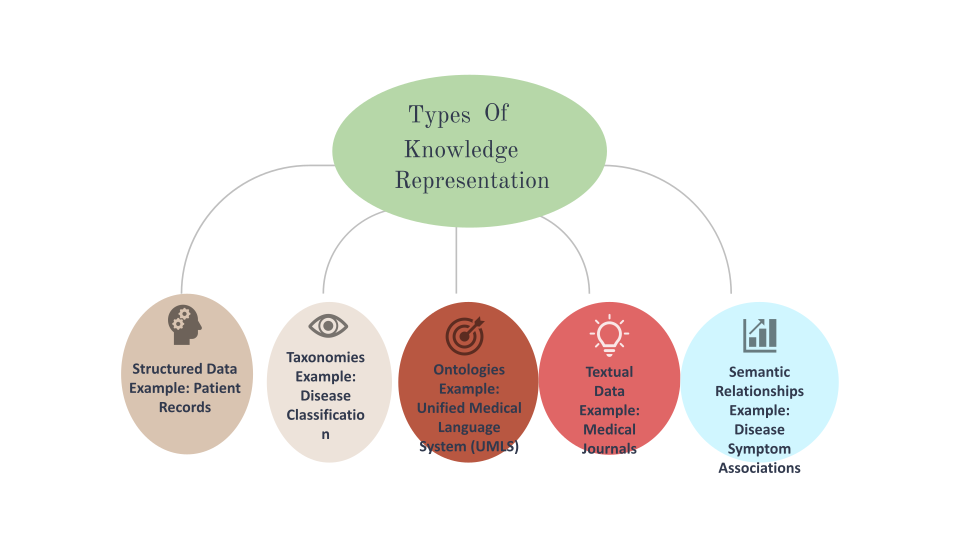
\includegraphics[width=0.95\textwidth]{images/types.png}
	\end{center}
	\caption{Types of Knowledge Representation}\label{fig:types}
\end{figure}

\subsection{Taxonomies}

\textbf{Definition}: Taxonomy is a hierarchical classification model that is
used to categorize entities/objects based on their similarities and
differences.

\textbf{Example}

\textbf{Disease Taxonomies}:

Taxonomies organize diseases and medical conditions based on the hierarchy of
diseases and affected organ systems. Disease classifications assist in patient
condition analysis, support clinical decision, and disease management,
enhancing patient care and outcomes.

\subsection{Ontologies}

We need structured mechanisms to derive relationships, concepts, and logic.
Ontologies allow us to store and represent concepts and their relationships
within a given domain.

\textbf{Ontologies in Familial History}:

When a patient like John visits a healthcare provider and mentions his family's
medical history, ontologies play a crucial role in organizing and utilizing
this information. For example, John might mention that his father had diabetes
and his mother had cardiovascular disease. An ontology designed for familial
history would define relationships between family members, genetic
predispositions, and medical conditions. By annotating John's family history
data according to this ontology, it becomes semantically interoperable.
Healthcare providers can then assess John's risk factors for certain medical
conditions based on his familial history, guiding preventive measures and
treatment decisions. Additionally, aggregating familial history data using
standardized ontologies enables population-level analysis and research, leading
to a better understanding of genetic patterns and more effective healthcare
strategies.

\subsection{Textual Data}

A lot of data such as clinical notes, medical literature, research papers,
etc., are in text-based formats which are unstructured and may contain hidden
patterns and context. This data requires Natural Language Processing (NLP) for
it to be fully utilized and extract relevant info such as patients' medical
context, or research findings, or expert opinions, and historical
moves/comments about a similar situation.

\section[Applications of Knowledge Representation]{Applications of \\Knowledge Representation}

Certainly, here are five applications of knowledge representation with concise
explanations:

\begin{enumerate}
  \item \textbf{Robotics}: Robots need to understand their environment; this
    allows them to perform tasks and collaborate with humans. Knowledge
    representation techniques allow robots to represent this data efficiently.

  \item \textbf{Knowledge Management}: Many systems need information from
    various sources, with different formats. Using ontologies and knowledge
    graphs allows these systems to use this data efficiently and make decisions
    based on them.

  \item \textbf{Recommendation Systems}: Using knowledge representation
    techniques such as knowledge graphs, a recommendation system uses various
    attributes for recommending different products, services, or content such
    as movies and series.
\end{enumerate}

\chapter{Knowledge Representation in Cognitive Systems}

As discussed in the previous chapter, Knowledge is data that has been given
structure and can be used in the future. Knowledge representation is a crucial
part of any cognitive system. The knowledge base, where all this knowledge is
stored in such a way that it is interlinked, and their relationship between the
data is clearly mentioned. Cognitive systems continuously learn with experience
and from the environment, hence a knowledge base system for it must support
\textbf{Continuous Learning}.

\section{Data Collection and Storage Strategies for Cognitive Systems}

Data is the fundamental building block, as discussed in Chapter 3. Cognitive
systems collect this data from various sources such as sensors, existing
databases, paid/free public APIs, web scraping, and crowdsourcing.

\subsection{Data Collection}

Using the example of a healthcare Cognitive system, let's see how these various
sources contribute to the data for the CS:

\begin{enumerate}
  \item \textit{Sensors}: Metrics like heart-rate, blood pressure, and sleep
    patterns can be collected using wearable devices, which allow deeper
    insights into patients' health. Chronic diseases can be monitored in a much
    better way using devices such as continuous glucose monitors for diabetes.
  \item \textit{Existing Databases}: EHR and public patient databases allow
    hospitals and medical personnel to access medical history, running
    medication, and ongoing treatment resulting in faster and more efficient
    management of patient care.
  \item \textit{APIs (Application Programming Interfaces)}: Public APIs allow
    systems to collect data directly from third-party data providers and
    healthcare applications and devices.
  \item \textit{Web Scraping}: This technique allows systems to collect data
    from websites such as online medical journals, research papers, and medical
    publications.
  \item \textit{Crowdsourcing}: Platforms use forms and questionnaires to
    collect user data such as symptoms, doctor ratings/reviews, and experiences
    such as side effects to create an extensive knowledge base.
\end{enumerate}

After this data is collected, it needs to be cleaned and stored.

\subsection{Data Pre-processing}

This collected data needs to be processed before storing it in a knowledge
graph. This may include cleaning missing values, removing outliers,
normalization, and feature selection.

\subsection{Data Storage}

Following steps may be taken to store this data:

\begin{itemize}
  \item \textbf{Schema Matching}: A schema must be decided, and data needs to
    be fixed into it. A schema must be defined for each individual source. This
    can be done by mapping similar attributes together.
  \item \textbf{Semantic Analysis}: Data contains context and relationships
    among itself. This needs to be represented in the knowledge base to allow
    the cognitive system to find the correct entity and its relation with other
    data. For example, consider a clinical note that mentions a patient. The
    cognitive system must be able to understand this real-life entity as the
    patient it knows from its knowledge base. This would allow it to get all
    the related data to the patient themselves and better extract insights from
    the note.
\end{itemize}

\section{Knowledge Representation in Cognitive System Databases}

After data collection and preprocessing, it needs to be represented in the
cognitive system databases. This can be done in the following ways:

\begin{enumerate}
  \item \textbf{Semantic Representation}: Traditional databases like RDBMS
    cannot represent complex relationships and capture the context of the data.
    Hence, we need a semantic representation of the data using techniques such
    as Knowledge Graphs. For example, the relationship between disease,
    symptoms, and treatment may be stored in ontologies. This allows the
    cognitive systems to draw diseases from symptoms, find treatments allowing
    better care for the patients.
  \item \textbf{Custom Knowledge Schemas}: Custom schemas create a better way
    to organize knowledge to better utilize this knowledge. Taxonomies can be
    used to store familial data allowing to store and see what disease someone
    may be predisposed to because of their parents and grandparents.
  \item \textbf{Multi-format Data}: Various formats may be needed to store such
    as textual reports, Medical images such as X-Rays MRIs etc. Patient's
    medical reports, X-rays, and other reports need to be stored along with
    their diagnosis; this is done using vector embedding, deep learning
    Techniques.
\end{enumerate}

\section{Enabling Continuous Learning in Cognitive Systems}

Healthcare is an ever-growing industry; every day new research, diseases,
treatments, and medications are found, hence we need to create a cognitive
system that can adapt to such an environment. Hence, we need to deploy adaptive
systems.

\begin{itemize}
  \item \textbf{Continuous Learning Algorithm}: Neural networks and other deep
    learning techniques are employed in cognitive systems, but these should be
    incrementally learning. That is, they should be able to update the
    knowledge base without requiring the model to retrain algorithms as an
    industry like healthcare is very dynamic. For example, a CS monitoring
    blood sugar should be able to learn new trends in blood sugar of patients
    to maintain accuracy hence the new data must be stored and learned
    incrementally.
  \item \textbf{Dynamic Memory Structure}: Traditional storage and memory
    architecture may become overwhelmed with the ever-growing data that is
    generated in real-time. Hence, we need a memory system that can handle and
    store the data based on its relevance, recency, and contextual importance.
    We may use priority-based storage systems witch store the recent data like
    recent patient history or symptoms based on the current case in the faster
    memory like cache. For example, patients that are currently admitted to the
    hospital, their data would be given more priority in the memory.
\end{itemize}

\section{Security Concerns}

Knowledge base and cognitive system databases store private data of users
(Medical data), important research papers, and other related data. To maintain
the privacy of users and prevent malicious entities from accessing the data,
security measures such as encryption, access control, and view management.

To maintain security and privacy of data and users can be done by following
methods:

\begin{itemize}
  \item \textbf{Encryption}: Methods like end-to-end encryption can be used to
    prevent accessing of data without authorization.
  \item \textbf{Minimal Data Collection}: The minimum amount of data, that is
    only necessary data for the functionality of the cognitive system should be
    collected from users.
  \item \textbf{Adding Noise while Storing Data}: Is done so that the data can
    still be used to train models but not make out any personal data.
  \item \textbf{Anonymization of Data}: Personal data of users must be
    protected to ensure that any data that is vulnerable should not contain
    users' personal details. This can also be done by differential privacy
    methods which use mathematical frameworks to ensure information about a
    specific person/user is not revealed.
  \item \textbf{Proper Access Control Mechanisms}: Role-based access control
    should be employed, i.e., people with certain roles/posts can only access
    certain data. For example, a doctor can access the data of a patient, but
    only when the patient is in the appointment with the doctor.
  \item \textbf{Auditing and Threat Detection}: Regular audits and security
    checks should be done to ensure that there is no suspicious activity
    happening. Threat detection should be done actively to detect any
    intrusions or attacks.
\end{itemize}

\chapter{Case Study - Knowledge Graphs}

A Knowledge Graph (KG), represents a collection of interlinked descriptions of entities - real-world objects, events, situations or abstract concepts. The entities are represented as nodes and the relationships between them as edges. The nodes and edges are labeled with attributes that describe the entities and relationships.

Just like any Graph, the KG is made up of nodes and edges, where the edges have a direction, indicating the direction of the relationship between a pair of concepts.

A KG is a structured representation of knowledge, which can be used understood as a `Graph of Concepts', to infer new knowledge, answer questions, and discover new relationships between entities. It is a powerful tool for representing and reasoning about complex relationships between entities in a domain.

\section{Knowledge Graphs in the Real World}

Knowledge Graphs are used in a variety of applications.
Any text corpus can be visualised in an interactive and intuitive
manner.

Graph Databases like Neo4j\cite{n4j}, Amazon Neptune\cite{neptune}, and JanusGraph\cite{janus} are a way to store and query data in the form of a graph. They are used in a variety of applications, including social networks, recommendation systems, fraud detection, and network analysis.

\section{Creating Knowledge Graphs using LLMs}

Large Language Models (LLMs) like GPT-3.5\cite{gpt3} and BERT\cite{bert} can be used to create Knowledge Graphs from unstructured text.
Through the use of fine-tuning and prompt engineering on a specific domain or dataset these models can be used to generate a KG from the text.

\subsection{Our Approach}

We use the Google's generative AI suite to access the `Gemini-1.0-pro' model to generate a
a structured representation of Knowledge Graph from a text corpus through a user given prompt or a
an already existing text corpus.

We use create tools to implement generation of KGs through function calling and
provide a user-friendly interface to interact with the model.


\subsection*{Examples}

Consider the following verse taken from the Hollow Knight game:\vspace*{1em}

\makeatletter
\renewcommand{\@chapapp}{}% Not necessary...
\newenvironment{chapquote}[2][2em]
{\setlength{\@tempdima}{#1}%
    \def\chapquote@author{#2}%
    \parshape 1 \@tempdima \dimexpr\textwidth-2\@tempdima\relax%
    \itshape}
{\par\normalfont\hfill--\ \chapquote@author\hspace*{\@tempdima}\par\bigskip}
\makeatother

\begin{chapquote}{\textit{The Pale King}}
    \noindent No cost too great.\\
    No mind to think.\\
    No will to break.\\
    No voice to cry suffering, \\[1em]
    Born of God and Void.\\
    You shall seal the blinding light that plagues their dreams.\\
    You are the Vessel.\\
    You are the Hollow Knight.
\end{chapquote}

This entire text can be converted into a Knowledge Graph, which can be used to
infer new knowledge, and discover new relationships between entities.

\pagebreak
\begin{figure}[h!]
    \centering
    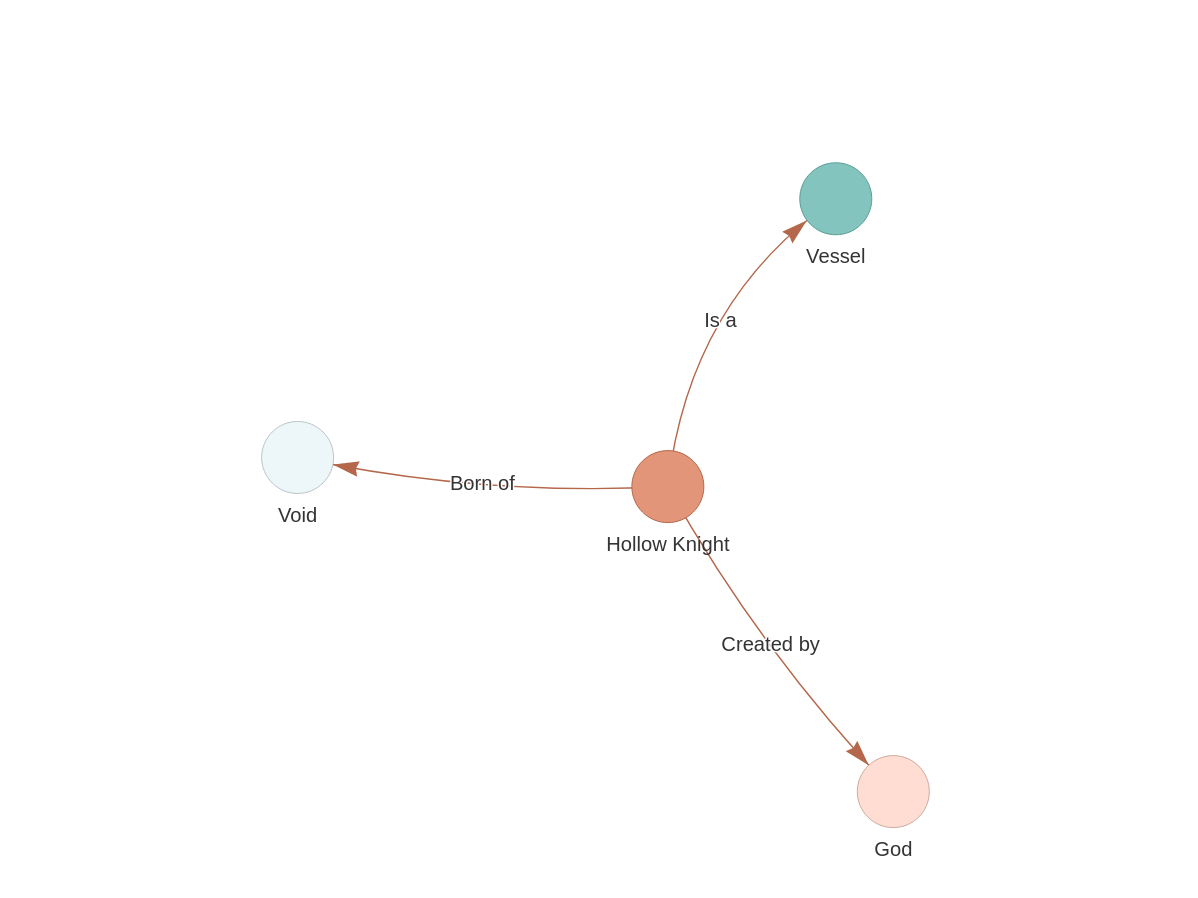
\includegraphics[width=0.9\textwidth]{images/hknobg.png}
    \caption{Corpus based Knowledge Graph}
    \label{fig:hk}
\end{figure}


Our approach\cite{korigamikkg} can also
create the following Knowledge Graph based on a user prompt:

\begin{verbatim}
User Prompt: "How does the Transformer model work?"
\end{verbatim}

Which generates the following Knowledge Graph:

\begin{verbatim}
Knowledge Graph:
{
    "name": "add_to_database",
    "args": {
        "entities": [
            {
                "description": "Neural network model for natural 
                language processing tasks",
                "type": "Model",
                "name": "Transformer Model Architecture"
            },
            ...
        ],
        "relationships": [
            {
                "to_entity_name": "Encoder",
                "relationship": "Composed of",
                "from_entity_name": "Transformer Model Architecture"
            },
            ...
        ]
    }
}

\end{verbatim}


The generated Knowledge Graph represents the relationships between the entities in the text, and can be used to answer questions, infer new knowledge, and discover new relationships between entities.

\begin{figure}[h!]
    \centering
    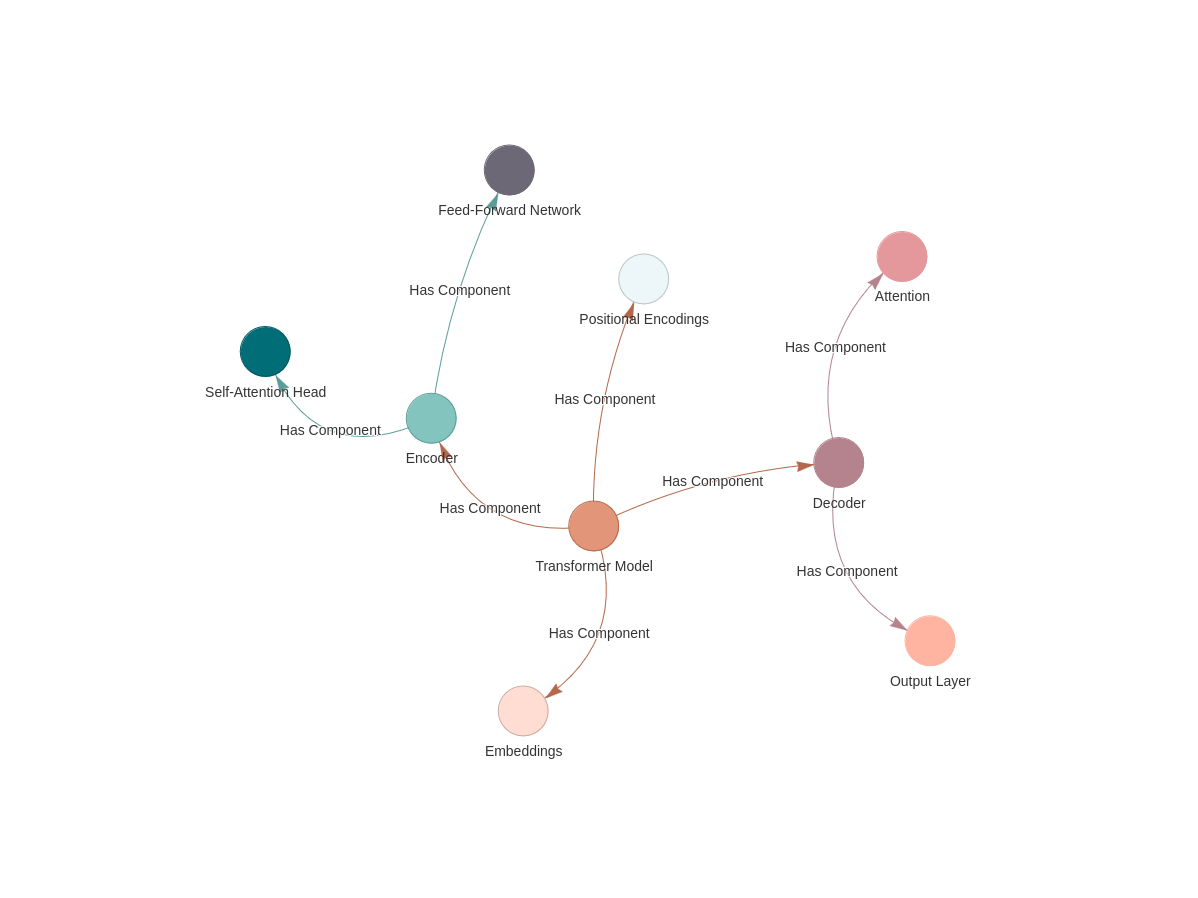
\includegraphics[width=0.9\textwidth]{images/transformer.png}
    \caption{Prompted Knowledge Graph: Transformer}
    \label{fig:kg}
\end{figure}

\section{Applications}

Knowledge Graphs have been used in  a slew of different industries and applications. These are used by researchers, marketing professionals, and data scientists to understand the relationships between entities in a domain, and to infer new knowledge from the data.

Recommendation systems and search engines use Knowledge Graphs to provide more relevant and accurate results to users. They can be used to answer questions, infer new knowledge, and discover new relationships between entities in a domain.

Inspite of these large scale applications, KGs can be used in a more personal and individual level. They can be used to create a personal knowledge base, to store and organize information, and to help you remember and recall information more easily.
They allow us to understand concepts at a glance and can be used to create a visual representation of a text corpus.



\chapter{Conclusion and emerging trends}

As we have shown, knowledge representation is a crucial aspect of cognitive
systems. It allows us to store, organize, and use data efficiently. Knowledge
representation techniques such as ontologies, taxonomies, and knowledge graphs
are used in various industries and applications. They help us understand the
relationships between entities in a domain, infer new knowledge from the data,
and discover new relationships between entities. Knowledge representation is a
rapidly evolving field, and we can expect to see more advancements in the
future.

\renewcommand{\bibname}{References}
\bibliography{refs}

\end{document}

